The Database layer provides an interface to store and retrieve data for the other layers. It helps maintaining the persistency and reliability of the data.

\begin{figure}[h!]
	\centering
 	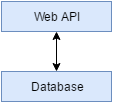
\includegraphics[width=0.60\textwidth]{images/database_layer}
 \caption{Example subsystem description diagram}
\end{figure}

\subsection{Web API}
The Web API allows access of data for clients

\subsubsection{Assumptions}
The Web API makes an assumption that bad calls will be ignored and security will not be needed.

\subsubsection{Responsibilities}
Web API should parse the html request.

\subsubsection{Subsystem Interfaces}

\begin {table}[H]
\caption {Subsystem interfaces} 
\begin{center}
    \begin{tabular}{ | p{1cm} | p{6cm} | p{3cm} | p{3cm} |}
    \hline
    ID & Description & Inputs & Outputs \\ \hline
    \#01 & HTML Interface & \pbox{3cm}{HTML Requests} & \pbox{3cm}{JSON Objects}  \\ \hline
    \#02 & Database Interface & \pbox{3cm}{JSON Objects} & \pbox{3cm}{JSON Objects}  \\ \hline
    \end{tabular}
\end{center}
\end{table}

\subsection{Database}
The Database provides routes to all data and stores the final data that is ready to be fetched by other layers.

\subsubsection{Assumptions}
The Database should only store valid data and ignore invalid data.

\subsubsection{Responsibilities}
The Database should store data and keep it ready to deliver to requesters.

\subsubsection{Subsystem Interfaces}
The database itself does not have any system interfaces.